\section{Zielsetzung}
\label{sec:Zielsetzung}

Das Ziel dieses Versuches ist die Untersuchung der Dipolrelaxation der 
strontiumdotierten Ionenkristalle Caesiumiodid und Kaliumbromid.
Dafür wird die Relaxationszeit $\tau(T,W,\tau_{\text{0}})$ der Dipole in den 
Kristallen bestimmt. Die Temperatur $T$ wird während des Versuches gemessen,
wogegen die Aktivierungsenergie $W$ und die charakteristische Relaxationszeit $\tau_{0}$
über den ebenfalls gemessenen Depolarisationsstrom berechnet werden können

\section{Theorie}
\label{sec:Theorie}

Die Dipolrelaxation wird in diesem Versuch an Ionenkristallen beobachtet.
Werden die Dipole der Kristalle durch ein äußeres elektrisches Feld aus ihrer 
Gleichgewichtslage ausgelenkt, benötigen sie eine Zeit um sich nach Abschalten des 
elektrischen Feldes wieder in ihre Ausgangslage zurück zubewegen. Der Übergang 
vom ausgelenkten Zustand zurück in den Ruhezustand wird als Relaxationsprozess 
bezeichnet. Die Dauer wird Relaxationszeit genannt.

\subsection{Dipole in Ionenkristalle}
\label{sec:Ionenkristalle}

Dieser Versuch wird an dem  Ionenkristalle Kaliumbromid durchgeführt.
Ein Ionenkristall ist durch seine Eigenschaft definiert, abwechselnd aus Anionen
und Kationen aufgebaut zu sein.
Kaliumbromid besitzt eine einfach kubische Kristallstruktur,
da die Kaliumkationen (\ce{K}: $4s^1$ $\to$ \ce{K+}: $3p^6$) und die Bromanionen 
(\ce{Br}: $4p^5$ $\to$ \ce{Br-}: $4p^6$)
jeweils eine flächenzentriet kubische Struktur besitzen, die 
um eine Gitterkonstante in eine Raumrichtung gegeneinander verschoben sind. 

abbildung Kristallstrukturen

Dadurch ist das Kriterium der abwechselnden Kationen-Anionen-Anordnung 
erfüllt. Ein solcher Ionenkristall ist durch diese regelmäßige Ionenanrdnung nach außen
elektrisch neutral. Um die Enstehung von Dipolen im Kristall zu ermöglichen wird 
die Probe mit einem Anteil von 0,005\% mit 
Stromtiumiodid (\ce{Sr++}: $4p^6$ , \ce{I-}: $5p^6$) dotiert. Da Strontiumiodid zweifach positiv 
geladene Strontiumionen enthält, entstehen Kaliumleerstellen, die mit der 
zusätzlichen positiven Ladung einen Dipol bilden, damit die Gesamtladungsneutralität des
Kristalls aufrechterhalten werden kann. 

abbildung Dipol

<<<<<<< HEAD
Ein Ionenkristall besteht aus alternierend negativ und positiv geladenen Ionen und ist nach außen somit neutral.
Wird ein solcher Kristall mit zweichfach geladenen Ionen dotiert entstehen Kationen-Leerstellen um die Ladungsneutralität aufrechtzuerhalten (Abb. \ref{fig:dipol}). 
||||||| merged common ancestors
Ein Ionenkristall besteht aus alternierend negativ und positiv geladenen Ionen und ist nach außen somit neutral.
Wird ein solcher Kristall mit zweichfach geladenen Ionen dotiert entstehen Kationen-Leerstellen um die Ladungsneutralität aufrechtzuerhalten (Abb. \ref{fig:dipol}). 
\begin{figure}
    \centering
    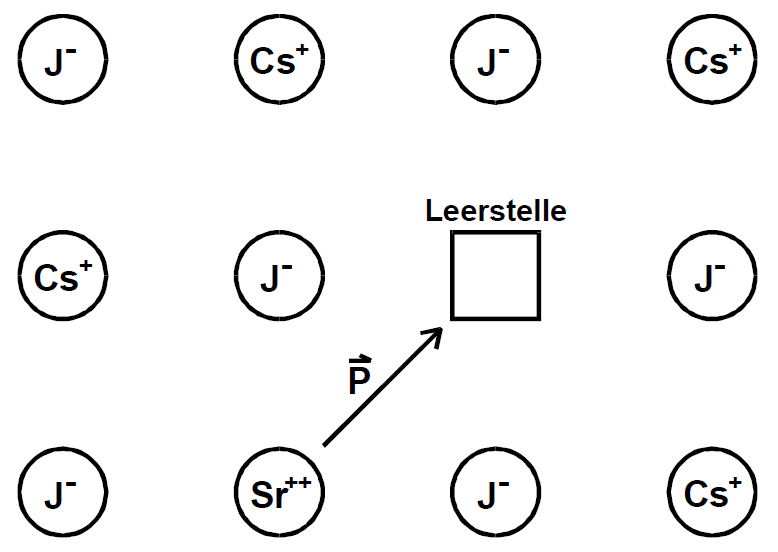
\includegraphics[width=0.5\linewidth]{img/Dipol.png}
    \caption{Entstehung eines elektrischen Dipols in einem Ionenkristall \cite{V48}.}
    \label{fig:dipol}
\end{figure}
=======
\subsection{Dipolpolarisation und -relaxation}
\label{sec:Dipolpolarisation}
>>>>>>> Theorie 1.0

Die Dipole, welche sich aus den Strontiumkationen und den Leerstellen ergeben, 
sind entsprechend ihrer Position im Gitter ausgerichtet. Da nur diskrete 
Gitterplätze möglich sind, ist auch die Richtungsverteilung der Dipole bei 
Raumtemperatur statistisch diskret verteilt. Eine Richtungänderung der 
Dipole ist durch Leerstellendiffusion möglich, wenn eine materialspezifische, 
thermische Energie überschritten wird. Sie wird Aktivierungsenergie $W$ genannt. 
Die Anzahl der Dipole deren Energie ausreichend zur Diffusion ist, ist durch die 
Boltzmann-Verteilung gegeben. Das heißt, wenn die spezifische Aktivierungsenergie 
überschritten wird  (Umgebungstemperatur muss ausreichend hoch sein), dann bewegen sich 
die Dipole zurück in ihre Ausgangslage. Die Relaxation beginnt. 
Je größer die Umgebungstemperatur, desto mehr Energie steht den Dipolen zur Verfügung 
und desto schneller relaxieren sie. Das heißt die Relaxationszeit 

\begin{equation}
    \tau(T) = \tau_0 \exp{\left(\frac{W}{k_\text{B}T}\right)}
    \label{eq1}
\end{equation}

wird mit steigender Temperatur kleiner. Die Bewegung der Ladungsträger während der 
Relaxation führt zu einem Strom innerhalb des Kristalls, welcher 
Depolarisationsstrom genannt wird. Dieser kann mit Strom durch
weitere bewegliche Ladungsträger (z.B. aufgrund von Störstellen) überlagert werden
(Untergrund).


\subsection{Berechnung der Aktivierungsenergie}
\label{sec:Aktivierungsenergie}

Um die Aktivierungsenergie zu bestimmen können zwei Ansätze verwendet werden,
wobei beide den Depolarisationsstrom beinhalten.
Der erste Ansatz wird über die Depolarisationsstromdichte
geführt. Dabei wird zunächst davon ausgegangen, dass diejenigen Dipole $y(T$), die 
sich durch ein angelgtes elektrisches Feld ausgreichtet haben durch 

<<<<<<< HEAD
Die Probe hat eine zylindrische Form und eine Dicke von etwa $\SIrange{3}{5}{\milli\meter}$ und dient als Dielektrikum in einem Plattenkondensator.
Um die Probe zu polarisieren, wird diese über einen Zeitraum $t_{\text{pol}} \gg \tau(T)$ einem elektrischen Feld $E$ ausgesetzt.
Im Mittel wird somit ein Bruchteil $y$ der Dipole in Feldrichtung weisen, welcher näherungsweise für $pE \ll k_\text{B} T$ als
\begin{equation}
    y(T) = \frac{p E}{3 k_\text{B} T} \label{y_t}
\end{equation}
beschrieben werden kann.
Anschließend wird die Probe auf eine Temperatur $T_0$ heruntergekühlt und der Polarisationszustand somit eingefroren.
Daraufhin wird das elektrische Feld abgeschaltet und die verbleibende Ladung durch kurzschließen des Kondensators entfernt.
Wird die Probe mit konstanter Heizrate
\begin{equation}
    b := \frac{\mathrm{d}T}{\mathrm{d}t} = \text{const}
\end{equation}
erhitzt, kehren die Dipole langsam in die statistische Richtungsverteilung zurück, was als Dipolrelaxation bezeichnet wird.
Dies induziert einen Depolarisationsstrom $j(t)$, welcher in Abhängigkeit von der Temperatur zunächst steil anwächst, ein Maximum durchläuft und anschließend wieder abnimmt (Abb. \ref{fig:pol_strom}).
Beschrieben werden kann $j(t)$ durch
||||||| merged common ancestors
Die Probe hat eine zylindrische Form und eine Dicke von etwa $\SIrange{3}{5}{\milli\meter}$ und dient als Dielektrikum in einem Plattenkondensator.
Um die Probe zu polarisieren, wird diese über einen Zeitraum $t_{\text{pol}} \gg \tau(T)$ einem elektrischen Feld $E$ ausgesetzt.
Im Mittel wird somit ein Bruchteil $y$ der Dipole in Feldrichtung weisen, welcher näherungsweise für $pE \ll k_\text{B} T$ als
\begin{equation}
    y(T) = \frac{p E}{3 k_\text{B} T} \label{y_t}
\end{equation}
beschrieben werden kann.
Anschließend wird die Probe auf eine Temperatur $T_0$ heruntergekühlt und der Polarisationszustand somit eingefroren.
Daraufhin wird das elektrische Feld abgeschaltet und die verbleibende Ladung durch kurzschließen des Kondensators entfernt.
Wird die Probe mit konstanter Heizrate
\begin{equation}
    b := \frac{\mathrm{d}T}{\mathrm{d}t} = \text{const}
\end{equation}
erhitzt, kehren die Dipole langsam in die statistische Richtungsverteilung zurück, was als Dipolrelaxation bezeichnet wird.
Dies induziert einen Depolarisationsstrom $j(t)$, welcher in Abhängigkeit von der Temperatur zunächst steil anwächst, ein Maximum durchläuft und anschließend wieder abnimmt (Abb. \ref{fig:pol_strom}).
\begin{figure}
    \centering
    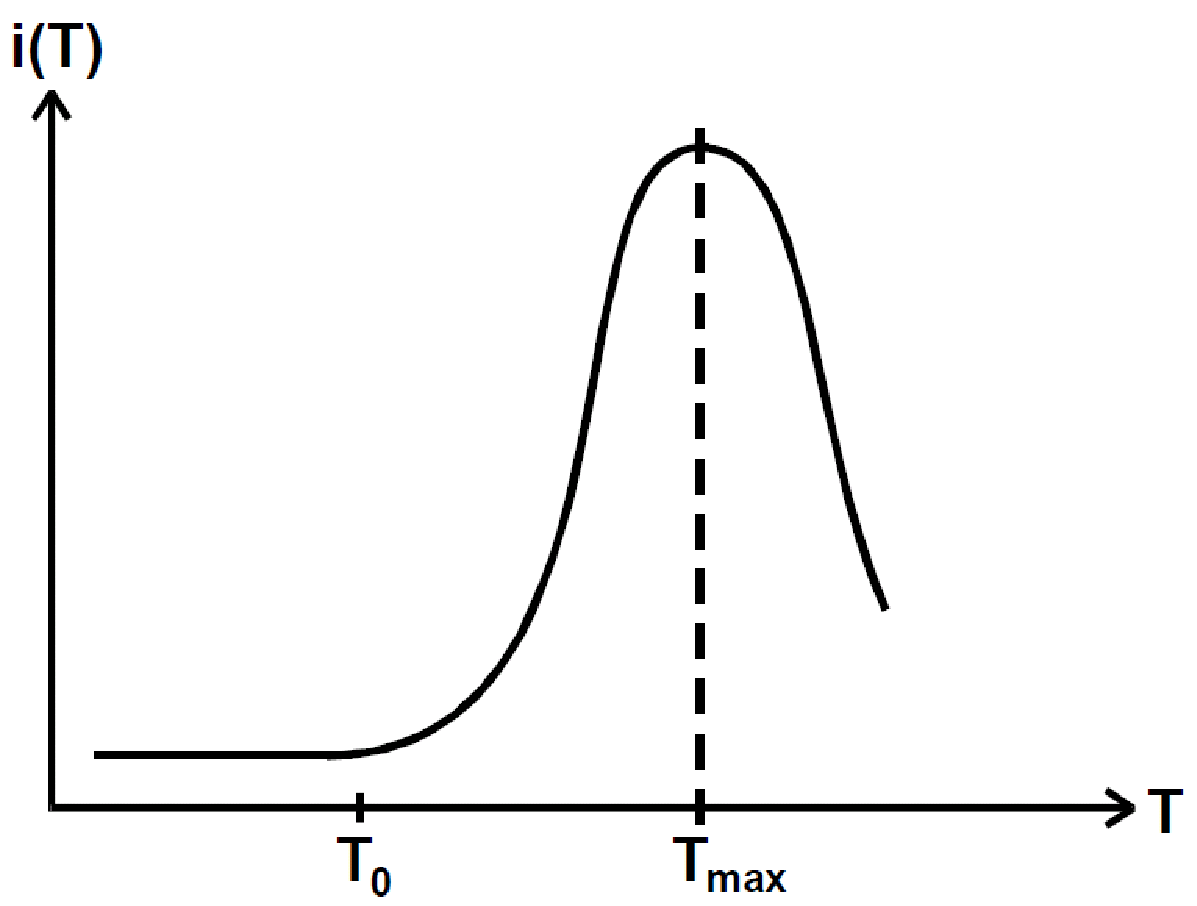
\includegraphics[width = 0.5\linewidth]{img/pol_strom.PNG}
    \caption{Der Polarisationsstrom in Abhängigkeit von der Temperatur \cite{V48}.}
    \label{fig:pol_strom}
\end{figure}
Beschrieben werden kann $j(t)$ durch
=======
>>>>>>> Theorie 1.0
\begin{equation}
    y(T) = \frac{p E}{3 k_{\text{B}} T} 
\end{equation}

gegeben sind. Der Depolarisationsstrom $j(t)$ kann dann über die ausgerichteten 
Dipole $y(T)$ über 

\begin{equation}
    j(t) = y(T_{\mathrm{P}}) p \frac{\mathrm{d}N}{\mathrm{d}t}
\end{equation}

ausgedrückt werden, wobei $p$ das Dipolmoment und 

\begin{equation}
    \frac{\mathrm{d}N}{\mathrm{d}t} = -\frac{N}{\tau(T)}
\end{equation}

die Stromdichte, also die pro Zeit und Volumeneinheit relaxierenden Dipole darstellt.
Eine Integration dieses Ausdrucks führt dann auf 

\begin{equation*}
    N = N_{\mathrm{P}} \exp{ \left( - \frac{ 1 }{ b } \int_{T_0}^T \frac{ \mathrm{d}T' }{ \tau(T') } \right )}
\end{equation*}

wobei $N_{\text{P}}$ die Anzahl der bereits zu Beginn des Relaxationsprozesses,
entsprechend des Gleichgewichtszustandes orientierten Dipole darstellt.
Die konstante Temperaturänderung ist definiert als

\begin{equation}
    b = \frac{\symup{d}T}{\symup{d}t}.
\end{equation}

Für den Depolarisationsstrom ergibt sich somit die Gleichung 

\begin{equation}
    j(T) = \frac{ p^{2} E }{ 3 k_{\mathrm{B}} T_{\mathrm{P}} } \frac{ N_{\mathrm{P}} }{ \tau_{\text{0}} } \exp{ \left( - \frac{ 1 }{ b \tau_{\text{0}} } \int_{T_{\text{0}}}^T \exp{ \left( - \frac{ W }{ k_{\mathrm{B}} T' } \right) \mathrm{d}T' } \right) } \exp{ \left( -\frac{ W }{ k_{\mathrm{B}} T } \right) } 
\end{equation}

wobei dieser Ausdruck für $T_{\text{0}} \approx T$ aufgrund des 
Zusammenhangs

\begin{equation*}
    \int_{T_{\text{0}}}^T \exp{ \left( - \frac{ W }{ k_{\mathrm{B}} T } \right )} \approx 0  
\end{equation*}

weiter zu 

\begin{equation}
    j(T) \approx \frac{ p^{2} E }{ 3 k_{\mathrm{B}} T_{\mathrm{P} }} \frac{ N_{\mathrm{P}} }{ \tau_{\text{0}} } \exp{ \left( - \frac{ W }{ k_{\mathrm{B}} T} \right ) }
    \label{eq2}
\end{equation}

approximiert werden kann.
Aus diesem Ergebnis kann schließlich die Aktivierungsenergie $W$ abgeleitet werden.
Eine weitere Möglichkeit zur Bestimmung von $W$ liegt in einem Ansatz der über 
die Polarisation $P$ geführt wird.
Die zeitliche Ableitung der Polarisation ist als

\begin{equation*}
    \frac{\mathrm{d}P}{\mathrm{d}t} = - \frac{ P(t) }{ \tau(T(t))}
\end{equation*}

gegeben, wobei sie einen Strom durch den Probenquerschnitt $F$ erzeugt und daher auch als

\begin{equation*}
    \frac{\mathrm{d}P}{\mathrm{d}t} = \frac{j(t)}{F} \qquad.
\end{equation*}

geschrieben werden kann.
Somit lassen sich die oberen Gleichungen auf die Form 

\begin{equation*}
    \tau(T) = \frac{ \int_{T}^\infty j(T') \mathrm{d}T' }{ b j(T) } 
\end{equation*}

bringen. Wenn $\tau(T)$ durch Gleichung \eqref{1} ersetzt wird kann 
schließlich die Aktivierungsenergie aus der Form 

\begin{equation}
    \frac{ W }{ k_{\mathrm{B}} T } = \ln{ \left( \frac{ \int_{T}^\infty j(T') \mathrm{d}T' }{ b j(T) \tau_{\text{0}} } \right) }
    \label{eq3}
\end{equation}

abgelesen werden. In der Praxis gilt
$j(T \to \infty) = j(T^*)  \approx 0$.

\cite{sample}
